\subsubsection{UC28 - Garage veicolo}
\begin{itemize}
	\item \textbf{Attori Primari}: utente autenticato;
	\item \textbf{Descrizione}: agli utenti autenticati è reso disponibile un Minigioco che consiste in un garage che dà la possibilità di effettuare modifiche ad un'auto sfruttando i premi ottenuti da:
	\begin{itemize}
		\item Progress Bar [UC17];
		\item Milestone Unlock [UC20];
		\item Lucky Spin [UC22];
		\item Leaderboard [UC24];
		\item Daily Rewards [UC26]. 
	\end{itemize} 
	Ogni pezzo ottenuto mostra un punteggio per ognuna delle seguenti informazioni:
	\begin{itemize}
		\item velocità;
		\item accelerazione;
		\item peso;
		\item maneggevolezza.
	\end{itemize}
	L'installazione di questi pezzi apporterà una modifica alle statistiche del veicolo che verranno visualizzate nella schermata principale del garage;
	\item \textbf{Scenario principale}: l'utente accede al Minigioco e visualizza un'auto base con la possibilità di modificarla attraverso due categorie:
	\begin{itemize}
		\item Prestazione [UC28.1];
		\item Estetica [UC28.2].
	\end{itemize}
	ogni modifica apportata viene automaticamente installata sull'auto.
	\item \textbf{Precondizione}: l'utente autenticato ha selezionato la voce \textit{Garage} dal menu dell'applicazione;
	\item \textbf{Post-condizione}: l'utente autenticato ha visualizzato la sua auto e installato le modifiche desiderate. 
\end{itemize}
\begin{figure}[h]
	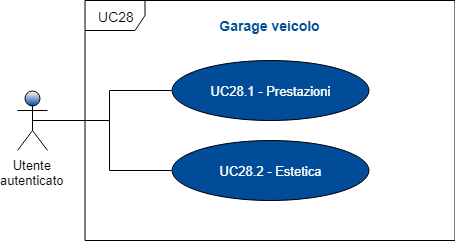
\includegraphics[width=10cm]{res/images/UC26-Garage.png}
	\centering
	\caption{UC28 - Garage veicolo}
\end{figure}
\newpage
\subsubsection{UC28.1 - Prestazione}
\begin{figure}[h]
	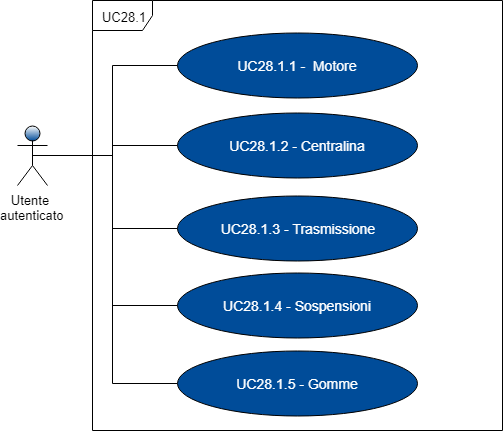
\includegraphics[width=9.5cm]{res/images/UC26-1Prestazioni.png}
	\centering
	\caption{UC28.1 - Prestazione}
\end{figure}
\begin{itemize}
	\item \textbf{Attori Primari}: utente autenticato;
	\item \textbf{Descrizione}: l'utente accede alla categorie di modifiche sulla prestazione per la propria auto. Avrà a disposizione un insieme di pezzi per ogni singola sottocategoria;
	\item \textbf{Scenario principale}: l'utente sta visualizzando la sua auto con una serie di modifiche da attuare per la categoria \textit{Prestazione} quali:
	\begin{itemize}
		\item motore [UC28.1.1];
		\item centralina [UC28.1.2];
		\item trasmissione [UC28.1.3];
		\item sospensioni [UC28.1.4];
		\item gomme [UC28.1.5].
	\end{itemize}
	\item \textbf{Precondizione}: l'utente ha intenzione di modificare la parte prestazionale della sua auto;
	\item \textbf{Postcondizione}: l'utente ha modificato gli elementi prestazionali della sua auto.
\end{itemize}
\subsubsection{UC28.1.1 - Motore}
\begin{itemize}
	\item \textbf{Attori Primari}: utente autenticato;
	\item \textbf{Descrizione}: in questa sezione l'utente può modificare il motore della propria auto se è in possesso di pezzi ricevuti da premi per il completamento degli obiettivi previsti dall'applicazione, dai premi giornalieri oppure sbloccabili al raggiungimento di un determinato livello esperienza grazie ad un continuo utilizzo dell'applicazione.
	All'inizio viene messo a disposizione il modello base;
	\item \textbf{Scenario principale}: l'utente vuole modificare il motore della propria auto e verificare la presenza di motori migliori da poter installare. Per pezzi non ancora sbloccati sarà possibile solo visualizzare i loro punti statistica mentre la foto del pezzo sarà oscurata;
	\item \textbf{Precondizione}: l'utente ha scelto di modificare il motore del proprio veicolo; 
	\item \textbf{Postcondizione}: l'utente ha correttamente scelto un motore sbloccato da installare, in caso contrario terrà il modello base.
\end{itemize}
\subsubsection{UC28.1.2 - Centralina}
\begin{itemize}
	\item \textbf{Attori Primari}: utente autenticato;
	\item \textbf{Descrizione}: in questa sezione l'utente può modificare la centralina della propria auto se è in possesso di pezzi ricevuti da premi per il completamento degli obiettivi previsti dall'applicazione, dai premi giornalieri oppure sbloccabili al raggiungimento di un determinato livello esperienza grazie ad un continuo utilizzo dell'applicazione.
	All'inizio viene messo a disposizione il modello base;
	\item \textbf{Scenario principale}: l'utente vuole modificare la centralina della propria auto e verifica la presenza di centraline migliori da poter installare, ma per pezzi non ancora sbloccati sarà possibile solo verificare i punti sulle statistiche oscurando l'immagine del pezzo stesso;
	\item \textbf{Precondizione}: l'utente ha scelto di modificare la centralina del proprio veicolo; 
	\item \textbf{Postcondizione}: l'utente ha correttamente scelto una centralina sbloccata da installare, in caso contrario terrà il modello base.
\end{itemize}
\subsubsection{UC28.1.3 - Trasmissione}
\begin{itemize}
	\item \textbf{Attori Primari}: utente autenticato;
	\item \textbf{Descrizione}: in questa sezione l'utente può modificare la trasmissione della propria auto se è in possesso di pezzi ricevuti da premi per il completamento degli obiettivi previsti dall'applicazione, dai premi giornalieri oppure sbloccabili al raggiungimento di un determinato livello esperienza grazie ad un continuo utilizzo dell'applicazione.
	All'inizio viene messo a disposizione il modello base;
	\item \textbf{Scenario principale}: l'utente vuole modificare la trasmissione della propria auto e verifica la presenza di pezzi di trasmissione migliori da poter installare, ma per pezzi non ancora sbloccati sarà possibile solo verificare i punti sulle statistiche oscurando l'immagine del pezzo stesso;
	\item \textbf{Precondizione}: l'utente ha scelto di modificare la trasmissione del proprio veicolo; 
	\item \textbf{Postcondizione}: l'utente ha correttamente scelto una trasmissione sbloccata da installare, in caso contrario terrà il modello base.
\end{itemize}
\subsubsection{UC28.1.4 - Sospensioni}
\begin{itemize}
	\item \textbf{Attori Primari}: utente autenticato;
	\item \textbf{Descrizione}: in questa sezione l'utente può modificare le sospensioni della propria auto se è in possesso di pezzi ricevuti da premi per il completamento degli obiettivi previsti dall'applicazione, dai premi giornalieri oppure sbloccabili al raggiungimento di un determinato livello esperienza grazie ad un continuo utilizzo dell'applicazione.
	All'inizio viene messo a disposizione il modello base;
	\item \textbf{Scenario principale}: l'utente vuole modificare le sospensioni della propria auto e verifica la presenza di sospensioni migliori da poter installare, ma per pezzi non ancora sbloccati sarà possibile solo verificare i punti sulle statistiche oscurando l'immagine del pezzo stesso;
	\item \textbf{Precondizione}: l'utente ha scelto di modificare le sospensioni del proprio veicolo; 
	\item \textbf{Postcondizione}: l'utente ha correttamente scelto le sospensioni sbloccate da installare, in caso contrario terrà il modello base.
\end{itemize}
\subsubsection{UC28.1.5 - Gomme}
\begin{itemize}
	\item \textbf{Attori Primari}: utente autenticato;
	\item \textbf{Descrizione}: in questa sezione l'utente può modificare le gomme della propria auto se è in possesso di pezzi ricevuti da premi per il completamento degli obiettivi previsti dall'applicazione, dai premi giornalieri oppure sbloccabili al raggiungimento di un determinato livello esperienza grazie ad un continuo utilizzo dell'applicazione.
	All'inizio viene messo a disposizione il modello base;
	\item \textbf{Scenario principale}: l'utente vuole modificare le gomme della propria auto e verifica la presenza di gomme migliori da poter installare, ma per pezzi non ancora sbloccati sarà possibile solo verificare i punti sulle statistiche oscurando l'immagine del pezzo stesso;
	\item \textbf{Precondizione}: l'utente ha scelto di modificare le gomme del proprio veicolo; 
	\item \textbf{Postcondizione}: l'utente ha correttamente scelto le gomme sbloccate da installare, in caso contrario terrà il modello base.
\end{itemize}
%\newpage
\subsubsection{UC28.2 - Estetica}
\begin{figure}[h]
	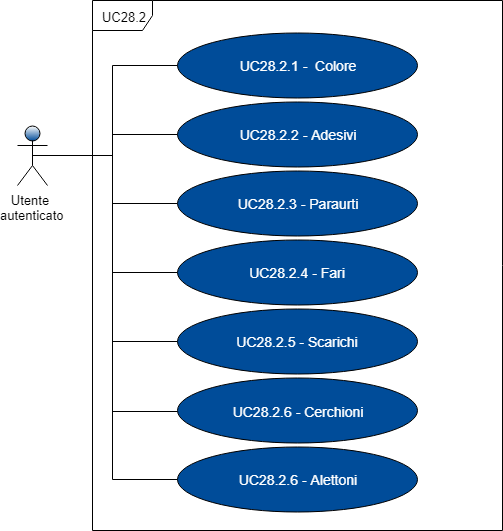
\includegraphics[width=9cm]{res/images/UC26-2Estetica.png}
	\centering
	\caption{UC28.2 - Estetica}
\end{figure}
\begin{itemize}
	\item \textbf{Attori Primari}: utente autenticato;
	\item \textbf{Descrizione}: l'utente accede alla categorie di modifiche sull'estetica per la propria auto. Avrà a disposizione un tot di materiale per ogni singola sottocategoria;
	\item \textbf{Scenario principale}: l'utente sta visualizzando la sua auto con una serie di modifiche da attuare per la categoria \textit{Estetica} quali:
	\begin{itemize}
		\item colore [UC28.2.1];
		\item adesivi [UC28.2.2];
		\item paraurti [UC28.2.3];
		\item fari [UC28.2.4];
		\item scarichi [UC28.2.5];
		\item cerchioni [UC28.2.6];
		\item alettoni [UC28.2.7].
	\end{itemize}
	\item \textbf{Precondizione}: l'utente ha intenzione di modificare la parte estetica della sua auto;
	\item \textbf{Postcondizione}: l'utente ha modificato gli elementi estetici della sua auto.
\end{itemize}

\subsubsection{UC28.2.1 - Colore}
\begin{itemize}
	\item \textbf{Attori Primari}: utente autenticato;
	\item \textbf{Descrizione}: in questa sezione l'utente può modificare il colore della propria auto se è in possesso di colori ricevuti da premi per il completamento degli obiettivi previsti dall'applicazione, dai premi giornalieri oppure sbloccabili al raggiungimento di un determinato livello esperienza grazie ad un continuo utilizzo dell'applicazione.
	All'inizio vengono messi a disposizione i colori complementari di base;
	\item \textbf{Scenario principale}: l'utente vuole modificare il colore della propria auto e verifica la presenza di colori migliori da poter installare, ma per quelli non ancora sbloccati sarà possibile solo verificare i nomi oscurando l'immagine del colore stesso;
	\item \textbf{Precondizione}: l'utente ha scelto di modificare il colore del proprio veicolo; 
	\item \textbf{Postcondizione}: l'utente ha correttamente scelto un colore sbloccato da installare, in caso contrario terrà quello base.
\end{itemize}
\subsubsection{UC28.2.2 - Adesivi}
\begin{itemize}
	\item \textbf{Attori Primari}: utente autenticato;
	\item \textbf{Descrizione}: in questa sezione l'utente può aggiungere l'adesivo alla propria auto se è in possesso di pezzi ricevuti da premi per il completamento degli obiettivi previsti dall'applicazione, dai premi giornalieri oppure sbloccabili al raggiungimento di un determinato livello esperienza grazie ad un continuo utilizzo dell'applicazione.
	All'inizio il veicolo non disporrà di nessun adesivo base;
	\item \textbf{Scenario principale}: l'utente vuole aggiungere un'adesivo alla propria auto e verifica la presenza di adesivi da poter installare, ma per pezzi non ancora sbloccati sarà possibile solo verificare i nomi oscurando l'immagine dell'adesivo stesso;
	\item \textbf{Precondizione}: l'utente ha scelto di aggiungere un adesivo al proprio veicolo; 
	\item \textbf{Postcondizione}: l'utente ha correttamente scelto un adesivo sbloccato da installare, in caso contrario terrà l'auto senza.
\end{itemize}
\subsubsection{UC28.2.3 - Paraurti}
\begin{itemize}
	\item \textbf{Attori Primari}: utente autenticato;
	\item \textbf{Descrizione}: in questa sezione l'utente può modificare il paraurti (anteriore e posteriore) della propria auto se è in possesso di pezzi ricevuti da premi per il completamento degli obiettivi previsti dall'applicazione, dai premi giornalieri oppure sbloccabili al raggiungimento di un determinato livello esperienza grazie ad un continuo utilizzo dell'applicazione.
	All'inizio viene messo a disposizione il modello base;
	\item \textbf{Scenario principale}: l'utente vuole modificare il paraurti (anteriore o posteriore) della propria auto e verifica la presenza di paraurti migliori da poter installare, ma per pezzi non ancora sbloccati sarà possibile solo verificare i punti sulle statistiche oscurando l'immagine del pezzo stesso;
	\item \textbf{Precondizione}: l'utente ha scelto di modificare il paraurti (anteriore o posteriore) del proprio veicolo; 
	\item \textbf{Postcondizione}: l'utente ha correttamente scelto un paraurti sbloccato da installare, in caso contrario terrà il modello base.
\end{itemize}
\subsubsection{UC28.2.4 - Fari}
\begin{itemize}
	\item \textbf{Attori Primari}: utente autenticato;
	\item \textbf{Descrizione}: in questa sezione l'utente può modificare i fari (anteriori e posteriori) della propria auto se è in possesso di pezzi ricevuti da premi per il completamento degli obiettivi previsti dall'applicazione, dai premi giornalieri oppure sbloccabili al raggiungimento di un determinato livello esperienza grazie ad un continuo utilizzo dell'applicazione. All'inizio viene messo a disposizione il modello base;
	\item \textbf{Scenario principale}: l'utente vuole modificare i fari (anteriori e posteriori) della propria auto e verifica la presenza di fari migliori da poter installare, ma per pezzi non ancora sbloccati sarà possibile solo verificare i nomi oscurando l'immagine del pezzo stesso;
	\item \textbf{Precondizione}: l'utente ha scelto di modificare i fari (anteriori e posteriori) del proprio veicolo; 
	\item \textbf{Postcondizione}: l'utente ha correttamente scelto i fari sbloccati da installare, in caso contrario terrà il modello base.
\end{itemize}
\subsubsection{UC28.2.5 - Scarichi}
\begin{itemize}
	\item \textbf{Attori Primari}: utente autenticato;
	\item \textbf{Descrizione}: in questa sezione l'utente può modificare gli scarichi della propria auto se è in possesso di pezzi ricevuti da premi per il completamento degli obiettivi previsti dall'applicazione, dai premi giornalieri oppure sbloccabili al raggiungimento di un determinato livello esperienza grazie ad un continuo utilizzo dell'applicazione.
	All'inizio viene messo a disposizione il modello base;
	\item \textbf{Scenario principale}: l'utente vuole modificare gli scarichi della propria auto e verifica la presenza di pezzi di scarico migliori da poter installare, ma per pezzi non ancora sbloccati sarà possibile solo verificare i nomi oscurando l'immagine del pezzo stesso;
	\item \textbf{Precondizione}: l'utente ha scelto di modificare gli scarichi del proprio veicolo; 
	\item \textbf{Postcondizione}: l'utente ha correttamente scelto gli scarichi sbloccati da installare, in caso contrario terrà il modello base.
\end{itemize}
\subsubsection{UC28.2.6 - Cerchioni}
\begin{itemize}
	\item \textbf{Attori Primari}: utente autenticato;
	\item \textbf{Descrizione}: in questa sezione l'utente può modificare i cerchioni della propria auto se è in possesso di pezzi ricevuti da premi per il completamento degli obiettivi previsti dall'applicazione, dai premi giornalieri oppure sbloccabili al raggiungimento di un determinato livello esperienza grazie ad un continuo utilizzo dell'applicazione.
	All'inizio viene messo a disposizione il modello base;
	\item \textbf{Scenario principale}: l'utente vuole modificare i cerchioni della propria auto e verifica la presenza di cerchioni migliori da poter installare, ma per pezzi non ancora sbloccati sarà possibile solo verificare i nomi oscurando l'immagine del pezzo stesso;
	\item \textbf{Precondizione}: l'utente ha scelto di modificare i cerchioni del proprio veicolo; 
	\item \textbf{Postcondizione}: l'utente ha correttamente scelto i cerchioni sbloccati da installare, in caso contrario terrà il modello base.
\end{itemize} 
\subsubsection{UC28.2.7 - Alettoni}
\begin{itemize}
	\item \textbf{Attori Primari}: utente autenticato;
	\item \textbf{Descrizione}: in questa sezione l'utente può aggiungere l'alettone alla propria auto se è in possesso di pezzi ricevuti da premi per il completamento degli obiettivi previsti dall'applicazione, dai premi giornalieri oppure sbloccabili al raggiungimento di un determinato livello esperienza grazie ad un continuo utilizzo dell'applicazione.
	All'inizio il veicolo non disporrà di nessun alettone base;
	\item \textbf{Scenario principale}: l'utente vuole aggiungere l'alettone alla propria auto e verifica la presenza di alettoni migliori da poter installare, ma per pezzi non ancora sbloccati sarà possibile solo verificare i nomi oscurando l'immagine del pezzo stesso;
	\item \textbf{Precondizione}: l'utente ha scelto di aggiungere un alettone al proprio veicolo; 
	\item \textbf{Postcondizione}: l'utente ha correttamente scelto l'alettone sbloccato da installare, in caso contrario terrà l'auto senza.
\end{itemize} 
